%!BIB program = bibtex
\documentclass[9pt, twocolumn, twoside, lineno]{pnas-new}
% Use the lineno option to display guide line numbers if required.

% PNAS研究论文模板
\templatetype{pnasresearcharticle} % Choose template 
% {pnasresearcharticle} = Template for a two-column research article
% {pnasmathematics} %= Template for a one-column mathematics article
% {pnasinvited} %= Template for a PNAS invited submission
% \usepackage{cite}
\usepackage{url}	
% 文章标题:“流域尺度的水资源利用体系:过渡框架和发展困局”
\title{Identifying regime transitions for water governance at a basin scale}
\label{title}
% Use letters for affiliations, numbers to show equal authorship (if applicable) and to indicate the corresponding author
% 作者列表
\author[a, b]{Shuang Song}  % 宋爽,一作
\author[a, b]{Shuai Wang}  % 王老师,通讯
\author[c, d]{Xutong Wu}  % 武旭同
\author[e]{Yongping Wei} % 尉老师
\author[a, b, 1]{Bojie Fu}  % 傅老师

% 机构列表
\affil[a]{ % 北师大地表国重
	State Key Laboratory of Earth Surface Processes and Resource Ecology, 
	Faculty of Geographical Science, 
	Beijing Normal University, 
	Beijing 100875, 
	P.R. China
}
\affil[b]{ % 北师大地理学部
	Institute of Land Surface System and Sustainability, 
	Faculty of Geographical Science, 
	Beijing Normal University, 
	Beijing 100875, 
	P.R. China
}
\affil[c]{ % 北大城环
	College of Urban and Environmental Sciences, 
	Peking University, 
	Beijing 100871, 
	P.R. China
}
\affil[d]{ % 中科院生态中心
	State Key Laboratory of Urban and Regional Ecology, 
	Research Center for Eco-Environmental Sciences, 
	Chinese Academy of Sciences, 
	Beijing 100085, 
	P.R. China 
}
\affil[e]{ % 昆士兰大学
	School of Earth and Environmental Sciences, 
	The University of Queensland, 
	Brisbane 4067, 
	Australia
}

% Please give the surname of the lead author for the running footer
% 领衔作者
\leadauthor{Song} 

% Please add a significance statement to explain the relevance of your work
% PNAS特有的“Significance陈述”,用不超过120个字来说明研究的意义和亮点
\significancestatement{
\label{significance}
	% Authors must submit a 120-word maximum statement about the significance of their research paper written at a level understandable to an undergraduate educated scientist outside their field of speciality. The primary goal of the significance statement is to explain the relevance of the work in broad context to a broad readership. The significance statement appears in the paper itself and is required for all research papers.
	It is a well-known fact that development of human societies backs on water use.
	Therefore, as natural water cycle has been dominated by growing socio-economic processes towards a hydro-social water cycle, big river basins are roundly governed phase by phase for further water use. 
	We propose an integrated index to detect water governance regimes and applying it to the Yellow River Basin, a typical fast-changing basin in China.
	Three water governance regimes are identified (massive supply, purpose turned, and all-sided governance), and a widespread regime-transition schema can be summarized after then. 
	By linking the transition with major water governance challenges, the schema can be a useful guideline for big river basins all around the world in their sustainability. 
}

% Please include corresponding author, author contribution and author declaration information
\authorcontributions{ % 作者的相应贡献
	Shuai Wang and Bojie Fu designed this research,
	Shuang Song performed the research and analysed data,
	Shuang Song, Xutong Wu wrote the paper.
	Yongping Wei reviewed the manuscript and proposed major useful advices.
}
\authordeclaration{ % 利益冲突陈述
	The authors declare no competing interests.
}

% 如果有共同一作的情况,则uncomment下面这行代码的注释
%\equalauthors{\textsuperscript{1}A.O.(Author One) contributed equally to this work with A.T. (Author Two) (remove if not applicable).}

% 通讯作者信息
\correspondingauthor{\textsuperscript{1}To whom correspondence should be addressed. E-mail: shuaiwang@bnu.edu.cn}

% 关键词,三到五个
% At least three keywords are required at submission. Please provide three to five keywords, separated by the pipe symbol.
\keywords{Regime shifts $|$ Water use $|$ Water governance $|$ Transformation $|$ Sustainability} 

%tag 摘要
% 为了
\begin{abstract}
	\label{abstract}
	% 为了持续的社会经济发展,人类治理了大型河流,并在世界范围内引发了一系列流域尺度的稳态转换。
	For water uses in sustaining socio-economic development, human have governed large rivers and led a transformation towards a hydro-social water cycle within basins all around the world. 
	% 由于水治理制度决定谁、何时和如何获得水,因此确定其过渡对于指导有效和可持续的用水至关重要。
	Since water governance regime decides who gets what water, when and how much, identification for its changes is critical to guiding efficient and sustainable water uses.
	% 在这里,考虑到水治理的三个主要维度(压力、供应和分配),我们开发了一个流域尺度上的综合水治理指数(IWGI),以检测制度的变化。
	Here, combining three main dimensions (supply, purpose and allocation), we develop an Integrated Water Governance Index (IWGI) to detect regime shifts of water governance at a basin scale.
	% 将该指数应用于典型的快速变化的流域——中国黄河流域,描绘了由环境、经济、社会和政治变化引起的长达半个世纪的三种水治理制度(大规模供应制度、目的性转向制度、全方位治理制度)之间的变迁。
	By applying the index to a typical rapid-changing basin -the Yellow River Basin, China, shifts between three water governance regimes (massive supply regime, purpose turned regime, all-sided governance regime) throughout half a century are well painted, which were caused by environmental, economic social and political changes.
	% 在此基础上,我们总结了一个与水社会循环相对应的一般制度变迁模式。
	Based on that, we summarize a widespread transition schema of water governance regimes, paralleled with a transformative trajectory towards hydro-social water cycle in the Anthropocene.
	% 由于资源挑战和结构挑战主要困扰不同制度下的水治理,这一过渡模式可以作为协调大流域治理的有益指导。
	Since different governance challenges mainly occurred at different phases in transition, this schema can be a useful guideline for governing big river basins in a coordinated way.
\end{abstract}


\dates{This manuscript was compiled on \today}
\doi{\url{www.pnas.org/cgi/doi/10.1073/pnas.XXXXXXXXXX}}


\begin{document}

\maketitle
\thispagestyle{firststyle}
\ifthenelse{\boolean{shortarticle}}{\ifthenelse{\boolean{singlecolumn}}{\abscontentformatted}{\abscontent}}{}
% If your first paragraph (i.e. with the \dropcap) contains a list environment (quote, quotation, theorem, definition, enumerate, itemize...), the line after the list may have some extra indentation. If this is the case, add \parshape=0 to the end of the list environment.

\label{introduction-section-1}
% 作为“人类世行星戏剧的中心”, water 不仅对地球系统进程至关重要,而且还支持着人类社会的发展。
\dropcap{W}ater, at “the centre of the planetary drama of the Anthropocene”, is not only essential for earth system processes, but also supporting development of human societies. 
%* add references
% 由于人类对水的依赖,人类活动深刻地改变了自然水循环,并逐步走向水-社会水循环。
Because of relying on water use, human activities have profoundly modified the natural water cycle and led a trajectory towards a hydro-social water cycle phase by phase
\cite{gleeson2020,sivapalan2012,qin2014,abbott2019,levia2020}.
% 面对这一重大转型,世界上许多大流域作为经济和文明热点,迫切需要成功的可持续治理
Facing this major transformation, many of the world's big river basins, also hot spots of economy and civilization, are urgently in need of successful water governance for sustainability
\cite{bestAnthropogenicStressesWorld2019,falkenmark2019,dibaldassarre2019}. 
% 水治理作为地球系统治理框架的重要组成部分,需要对人与水之间复杂的关系有深刻的理解。
As an integral part of a proposed earth system governance framework, water governance requires deep understanding of the complex relationships between human and water
\cite{biermann2012,steffen2020,dibaldassarre2019}
% 因此,识别流域尺度上由水-社会水循环转变引起的水治理变化至关重要。
Therefore, it is crucial to identify changes of water governance induced by the transformation towards hydro-social water cycle, especially at a basin scale.

\label{introduction-section-2}
% 缺乏治理就是缺乏可持续性
For water, missing governance means missing sustainability \cite{undpwatergovernancefacility2015}.
% 根据联合国开发计划署(UNDP)的说法,水管理决定了用水的三个关键方面:“有多少水可供使用?、“如何平衡用水服务?”“以及‘如何平等有效地分配水资源?’”
According to United Nations Development Programme (UNDP), three key dimensions are decided by water governance regime directly: ``How much water can be used? (supply)'', ``How to balances different water use services? (purpose)'' and ``How to allocate water equally and efficiently? (allocation)'' 
\cite{undpwatergovernancefacility2013,undpwatergovernancefacility2015,undpwatergovernancefacility2016}.
% 制度是系统结构和功能的一种稳定状态,其大规模的持续变化可能对系统结果产生实质性的影响,具有广泛的级联效应,即制度变迁.
Regime is a stable state of system’s structure and function, of which large and persistent changes may lead to huge impacts on the outcomes of system with widespread cascading effects 
\cite{rocha2018,gregr2020}.
% 因此,制度的转变是水治理发生实质性变化的信号,可能导致对可持续性的新挑战。
Defined as regime shifts, therefore, it is a signal of substantive changes in water governance and may lead to new challenges to sustainability 
\cite{steffen2020}.
% 然而,随着环境、经济、社会和政治方面的变革,水治理制度可以从上述每一个关键方面(供应、目的和分配)发生重大变化。
Along with environmental, economic, social and political changes, however, regime shifts of water governance can be triggered from each of the above key dimensions (supply, purpose, and allocation)
\cite{undpwatergovernancefacility2013,undpwatergovernancefacility2015,undpwatergovernancefacility2016}.
% 首先,受环境恶化和进一步经济增长对水的需求的影响,维持社会的水供应可能会因为缺水而面临压力,但治理政策(如修建水库)可能会有所帮助.
Firstly, effected by environment deteriorate and water demands of further economic growth, maintaining water supply for societies can be stressful because of scarcity, but policies (such as construction of reservoirs and channels) can be helpful
\cite{greveGlobalAssessmentWater2018, wada2017, qin2019}.
% 其次,在供应用水(如家庭用水和粮食生产用水)和非供应用水(如工业生产或能源用水)之间存在权衡,这需要由治理制度来平衡。
Secondly, there is trade-off between provisioning-purpose water services (such as domestic use and food production uses) and non-provisioning-purpose services (such as uses for industrial production or energy), which in need of weights through water governance
\cite{liu2017, florke2018}.
% 第三,由于配置是流域关注的问题,它不仅受到区域环境基础的影响,而且还受到区域经济比较优势的影响,而经济比较优势可能受到社会发展和政策的影响。
Thirdly, since governance concerns water allocation at the whole basin, it is not only influenced by regional environmental context, but also by regions' economic comparative advantages, which is easily altered by changing social and political
\cite{roobavannan2017,speed2013}.
% 综上所述,随着向以人为主导的水-社会水循环的转变,水治理制度由三个变化的维度(供应、目的和分配)决定,缺乏简单而全面的方法来确定制度变化,这对成功治理留下了关键的差距.
Taken together, along with the transformation towards a human-dominated hydro-social water cycle, water governance regimes are determined by three changing dimensions (supply, purpose and allocation). However, the lack of simple but comprehensive method in identifying changes of water governance regime leaves fatal gaps towards successful water governance for sustainability (Figure~\ref{fig:framework}).

\label{introduction-section-3}
% 黄河流域(YRB,详见方法S2)经历了中国最密集的用水和剧烈的制度变迁,从古代起就面临着水资源管理方面的非凡挑战。
The Yellow River Basin (YRB, see \textit{Appendix} Methods S1 and Figure S1 for details) had experienced the most intense water use and dramatic shifts of regime in China, with extraordinary challenges in water governance from the ancient time.
% 半个世纪前,黄河巨大的泥沙负荷不仅给黄河带来了灾难,也给黄河的用水带来了困难。
Half century ago, the huge sediment loads of the Yellow River not only brought disasters, but also made it difficult for water use 
\cite{song2020,li2020}. 
% 自20世纪60年代以来,通过实施养护措施、水库调蓄和堤防工程,这些问题得到了有效遏制。
Since 1960s, with implementations of conservation measures, regulation reservoirs, and levees constructions, these high-sediment-caused issues were effectively contained 
\cite{wang2016,wu2020}.
% 然而,由于过度用水,黄河的严重干涸带来了新的治理挑战,并推动了一系列相关政策(如调节用水和限制取水)来应对。
However, because of over water use, serious drying up of the Yellow River led new governance challenges and promoted a range of related policies (such as regulating water use and limiting water withdrawals) to deal with 
\cite{xia2012}.
% 今天,由于水的需求仍然难以完全满足,各区域和部门之间必须进行各种权衡,要取得成功的水治理还有很长的路要走。
Today, as water demands are still difficult to be completely met and various trade-offs must be involved between regions and sectors, there is still a long way towards successful water governance 
\cite{wang2019, wohlfart2016}.
% 总而言之,YRB是世界上变化最迅速的盆地,对由环境、经济、社会或政治因素引起的无休止的治理挑战作出各种各样的反应。
All in all, the YRB has been the most rapid-changing basins in the world, with myriad responses to the endless governance challenges induced by environmental, economic, social or political factors.
% 因此,确定YRB内的水管理制度变化可以为世界快速变化的大河流流域提供洞察,以应对可持续发展方面的挑战。
Therefore, identifying the regime shifts for water governance within YRB can provide crucial insights to the world's rapid-changing big river basins for meeting challenges towards sustainability.

\label{introduction-section-3}
% tag 引言最后一段
% 这里我们整合了三个方向,提出了描绘流域人水关系的指数
Here, based on three key dimensions (supply, purpose and allocation) of water governance, we develop an Integrated Water Governance Index (IWGI) to detect changes of water governance at a basin scale (Figure~\ref{fig:framework}).
% 使用案例研究
By applying the index to a typical rapid-changing big river basin (the YRB), we analysed the complicated regimes shifts of water governance and their main causes in a comprehensive but simple way.
% 最后总结出一般性框架
Finally, a general regime transition schema is summarized, which can be a practicable guideline for big river basins to governance in a coordinated way towards sustainability since it reveals widespread challenges regarding water governance.


\begin{figure*}%[htbp]
	\centering
	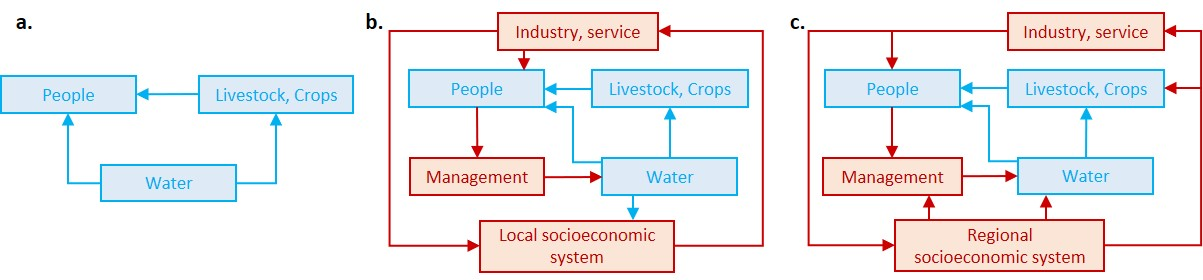
\includegraphics[width=0.8\linewidth]{../../figures/main/framework.jpg}
	\caption{
		A framework for understanding the relationship between transformation towards hydro-social cycle and transitional water governance regimes, with our main goal in detecting regime shifts by a simple and comprehensive index.
		% 图A是水资源利用的三个维度。每个维度都有两个极点(红色字表示),指示水资源利用在该轴上的两个变化方向。
		\textbf{A,} three key dimensions (supply, purpose and allocation) of water governance (see Methods for details). Each dimension has two poles (denoted in red) which indicate the two potential directions of changes along that axis: (1) ``supply'' shifts between scarcity and abundance. (2) ``purpose'' weighted between provisioning services or non-provisioning services. (3) ``allocation'' changes between balanced or lopsided. 
		% 图B是将三个维度结合后的变化情况。因上述三个维度随着社会发展而不断变化,其组合的水资源利用状态也不同。这个过程中当突变发生时,可能标志着水资源利用发生了稳态转换,因此我们需要一个指标来监测其变化。
		\textbf{B,} the governance changes combined the three dimensions. Because the above three dimensions change along with the trajectory towards hydro-social water cycle, combined water governance status is also various with that. When abrupt change occurs during this process, it may indicate a regime shift in water governance
		\cite{steffen2018,abbott2019,levia2020}.
	}
	\label{fig:framework}
\end{figure*}


\section*{Results}
\subsection*{Water governance regimes}

\begin{figure}[ht!]
	\centering
	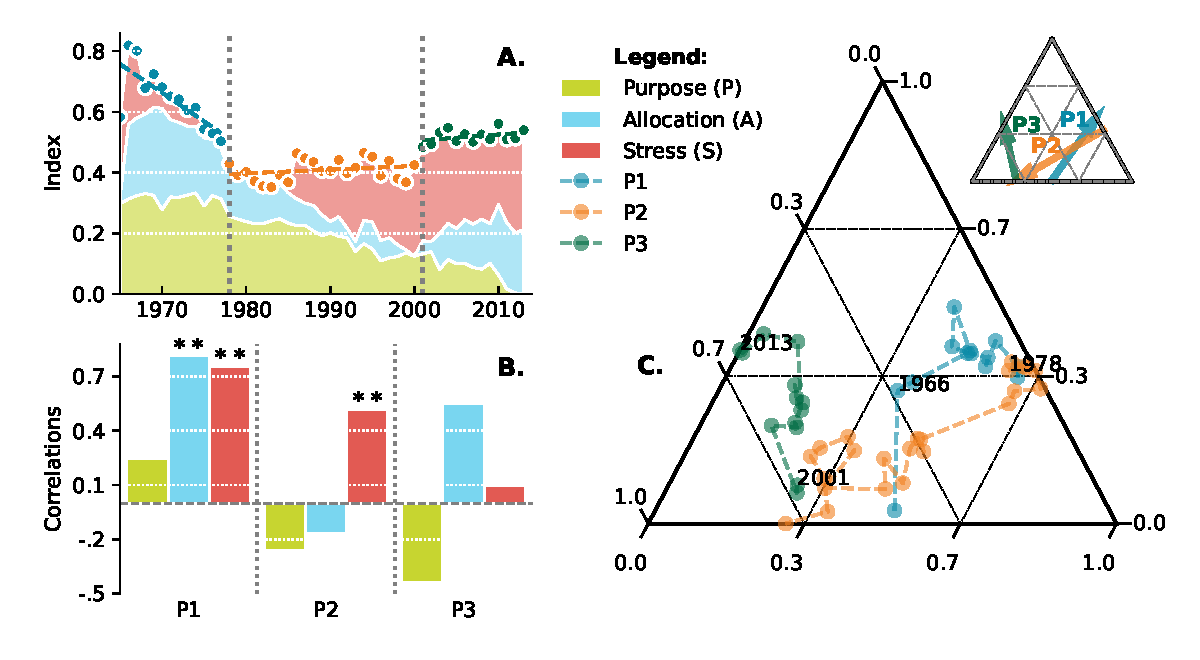
\includegraphics[width=\linewidth]{../../figures/main/index.pdf}
	\caption{Changes of the IWGI index. 
	\textbf{A,} Change points detection. With significant change points in 1978 and 1994, the IWGI have three different periods in changing trend.
	\textbf{B,} Contributions of each dimension to the changes of IWGI within three periods. Supply, purpose and allocation have made the main positive contributor of P1, P2 and P3, respectively.
	}
	\label{fig:IWGI}
\end{figure}

% 这一节主要展示IWGI的变化趋势和WUR的划分
With two significant points, the changes of IWGI are detected into three periods (Figure~\ref{fig:IWGI}A). 
Not only the slope of trends are various within each period, changes are also mainly contributed by different water governance dimensions (Figure~\ref{fig:IWGI}B).
% 第一阶段
In the first period (P1, 1965-1978), the IWGI was rapidly increasing and the supply made the most striking positive contribution (131\%), while purpose and allocation had slight negative contribution (-11\% and -20\%).
% 第二阶段
In the second period (P2, 1979-1994), though contributions of purpose and allocation turned into positive, the IWGI experienced a drop because huge-declined supply capacity plays a larger negative role (-188\% dropped than P1). 
% 第三阶段
However, as the further increasing of positive contributions of purpose (75\%) and allocation (84\%), and decreases of water supply in negative contribution (-59\%) in the third period (P3, 1995-2013), a positive growth of the IWGI returned.

\begin{figure}[!htbp]
	\centering
	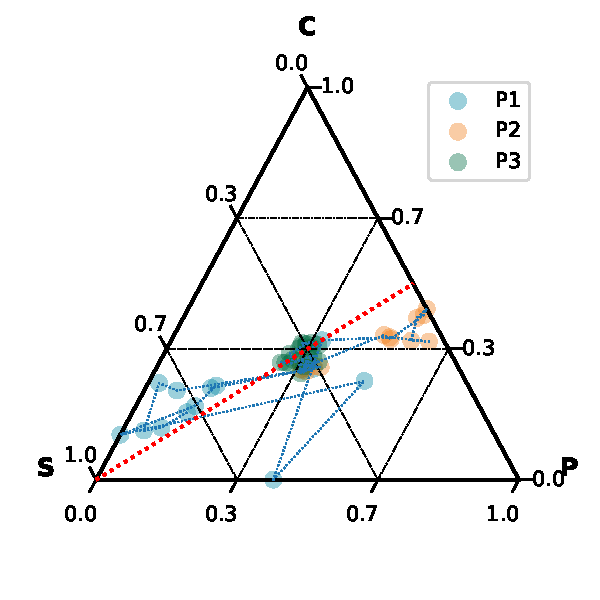
\includegraphics[width=0.9\linewidth]{../../figures/main/phases.pdf}
	\caption{Combination of contributions regards three dimensions in different periods (S: supply; P: purpose; A: allocation). The closer a point to an angle of the triangle, greater the proportion of the contribution of this dimension.
	The red indicator line in this ternary plot denotes 1:1 contributions between purpose (P) and allocation (A). When the points are bellow this line, the contribution ratio of allocation is lower than that of function, and vice versa.}
	% 由于阶段一的点位于该线上方,L的净贡献比例多于P,而第二阶段的点则恰好相反。
	\label{fig:phases}
\end{figure}

% 总而言之,每个阶段都由水资源利用的不同维度提供最大的正向作用
Taken together, each period has the unique most striking positive contributor to IWGI, and overall features of three dimensions in different periods are shown in Figure~\ref{fig:phases}.
% 第一阶段到第二阶段
Throughout the whole P1, water governance regime dominated by increasing supply capacities. After then, it experienced a shift to slow down in increasing supply during the P2, with a reverse in the contributed proportion between purpose and allocation, too.
% 第三阶段集中
Finally, the contribution of three dimensions were much similar in P3 (32.91\%, 31.87\% and 35.21\% for purpose, allocation and supply respectively), making the points highly concentrated at the centre of the ternary diagram.
% 总结来说,三个稳态
All in all, there were three water governance regimes corresponding three different periods: massive supply regime (P1: 1965-1978), purpose turned regime (P2: 1979-1993), all-sided governance regime (P3: 1994-2013). 

% tag 结果2
\subsection*{Causes of water governance regime shifts}
\label{result2}

\begin{figure}[th!]
	\centering
	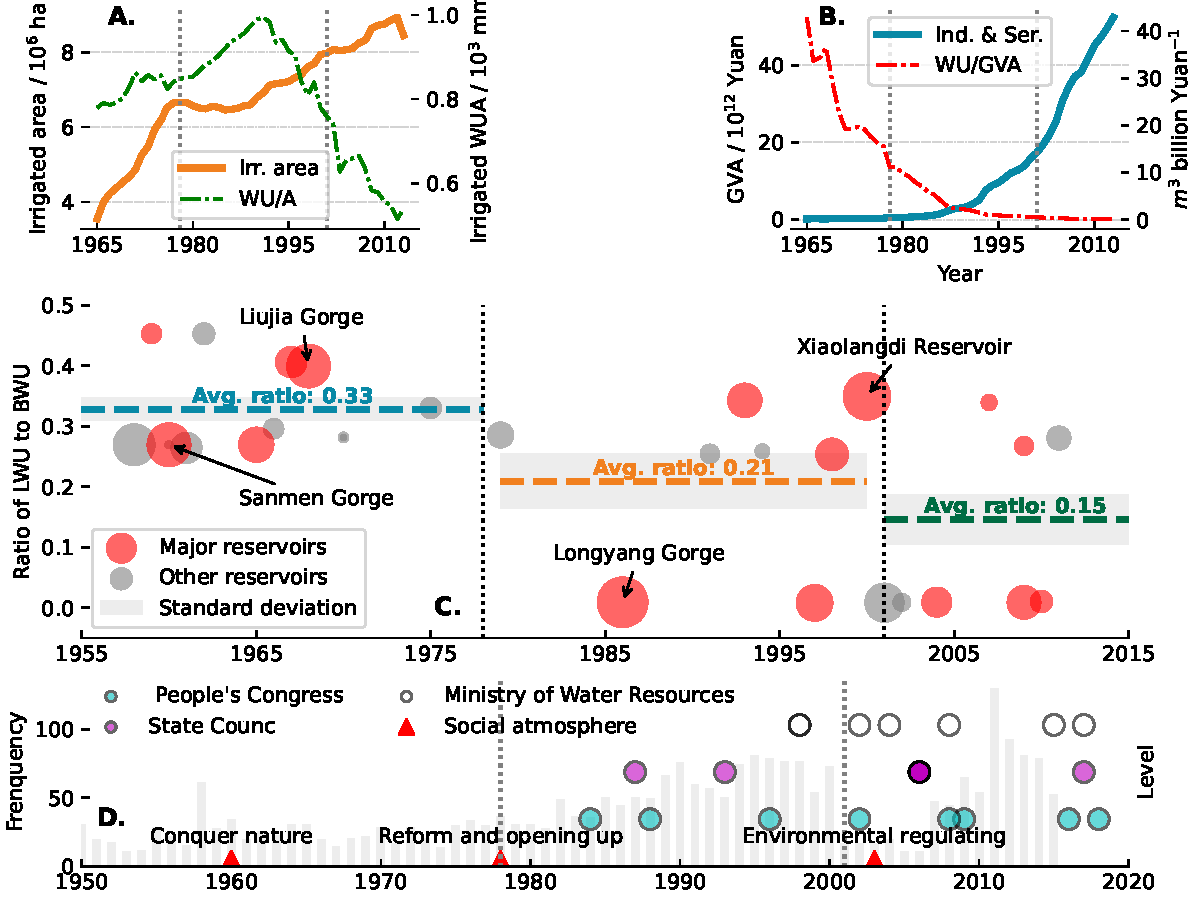
\includegraphics[width=\linewidth]{../../figures/main/causes.pdf}
	\caption{
		Causes of water governance regime shifts: environment changes, economic growths and efficiency changes, social transformation and water governance policies.
		\textbf{A.} Changes of total irrigated area, and water consumptions in per unit of area (\textit{SI Appendix} Methods S2).
		\textbf{B.} Changes of gross values added (GVA) of industry and services, and their water use intensity for unit production (WUI) respectively (\textit{SI Appendix} Methods S2).
		\textbf{C.} Completed time of each new reservoir and their located regions' water use percentages in basin's total water use (WU), at that time. Red ones denote hub reservoirs in the basin, which plays a role in basinal integrated water management. Size of the points indicates their magnitude of water storage capacities. Some important or special reservoirs' name denoted: (1) Xiaolangdi reservoir and Sanmen Reservoir were constructed mainly responsible for managing sediments of the Yellow River. (2) Liujia Gorge, Longyang Gorge, were constructed mainly responsible for managing water flood discharge and water supply. These marked reservoirs, therefore are more significant for the entire basin, rather than regional development.
		\textbf{D.} Social transformations and national levels' policies related to water governance (see \textit{SI Appendix} Methods S1 and Table S2). Four transformations are ``ethos of conquer nature (since 1958)'', ``reform and opening-up (since 1978)'', ``the 87 Water Diversion Scheme (since 1987)'', ``environmental regulation (since 2003)'' in order (see \textit{SI Appendix} Methods S1).
	}
	\label{fig:Causes}
\end{figure}

% 经济总量提升导致资源耗竭的加速。
Firstly, the expansion of irrigated area and the economic growth of industry and services are keys to the turn of purpose between P1 and P2. During the P1, irrigated agricultural area in the Yellow River basin expanded rapidly at a rate of $0.25*10^6 ha/yr$ (Figure\ref{fig:Causes} A), and irrigation water was the dominant water use ($81.56\%$ of the total water use in 1965, and $83.17\%$ in 1978, \textit{SI Appendix} Fig. S3). Entering P2, however, while the expansion of irrigated area stalled, industry and services gradually took off with more water demands (Figure\ref{fig:Causes} B), leading to $8\%$ reduction of proportion of irrigation water use (\textit{SI Appendix} S3).

% 用水关系的变化
Secondly, efficiency of water use changed from the P2 to the P3.
While irrigated area resumed expansion again in the P3 (Figure\ref{fig:Causes}A), both industry, urban services were boosting their economic role (represented by Gross Added Values, GVA) (Figure~\ref{fig:Causes}B). 
However, because of the improved water use efficiency by technology and water conservation practices (\textit{SI Appendix} Fig. S4), both of them experienced significant declines in water use intensity (WUI) for unit production (Figure~\ref{fig:Causes}A and Figure~\ref{fig:Causes}B). 
As a result, the differences between sectors of water use reduced while the total water consumption remains stable, during the P3 (\textit{SI Appendix} Fig. S3).

% 最后,环境背景、社会转型和水治理政策在这三个时期都发挥了作用。
Finally, environmental context, social transformation and water governance policies played roles throughout all three regimes. 
% 根据水库的位置,计算了各水库的区域用水量与盆地用水量之比。
According to locations, we calculate the ratios of regional and basinal water use for each reservoir (R/B ratio), and a higher ratio represents potential role for supply rather than regulating (Figure~\ref{fig:Causes}C).
% 在自然水资源相对丰富的P1年,水库大多建在需水量高的地区,水库的需水量比显著偏高。
Under the guide of ``ethos of conquer nature'', most of the reservoirs are built in regions with high water demands during the P1, when natural water resource is relatively abundant (\textit{SI Appendix} Fig. S5), as R/B ratios are significantly higher (Figure~\ref{fig:Causes}C, p<0.01). 
% 在P2中,新水库的数量显著减少,水量分配受到“87调水方案”的严格控制,总库容几乎没有增加(\textit{SI  Appendix}图S6)。
In the P2, the number of new reservoirs decreases significantly and allocation of water were rigorously controlled by ``the 87 Water Diversion Scheme'', with little increment of total water storage capacities (\textit{SI Appendix} Fig. S6). 
% 进入P3期后,以“环境监管”为指导的无数国家层面的水治理政策被提出,为了便于监管,新建的水库数量甚至更多,其中大部分建在R/B比较低的地区。
Entering the P3, myriad national-level water governance policies proposed under the guide of ``environmental regulation'' (Figure~\ref{fig:Causes}D), and the number of new reservoirs are even higher for facilitating regulating, most of which were built in regions with lower R/B ratio (Figure~\ref{fig:Causes}C and \textit{SI Appendix} Fig. S6).


% tag 讨论
\section*{Discussion}
\label{Discussion}

\subsection*{Water governance challenges along transition regimes}

\begin{figure*}[htbp!]
	\centering
	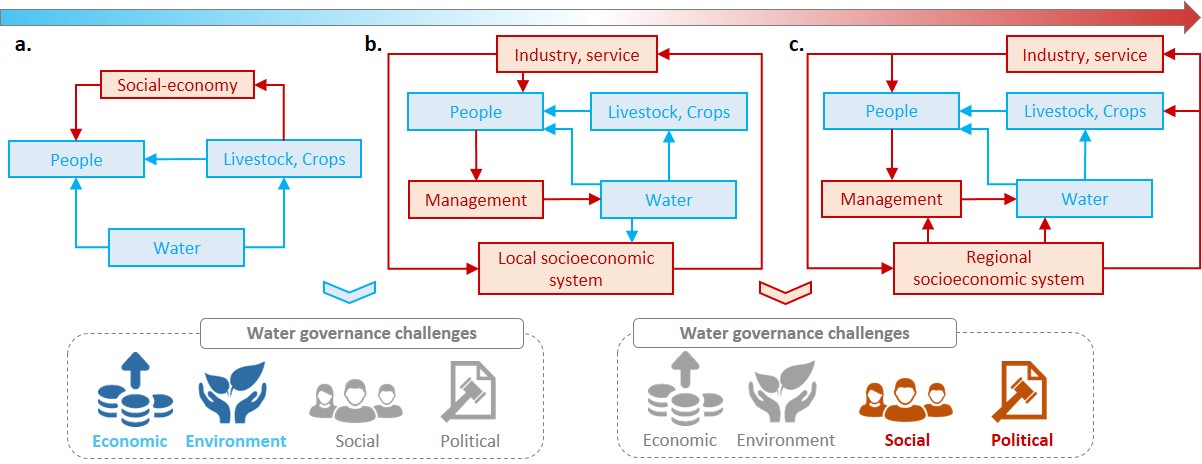
\includegraphics[width=0.8\linewidth]{../../figures/main/transition.jpg}
	\caption{
		Transition schema of water governance along with the transformation towards hydro-social water cycle. Blue pathways dominated by natural water loop while red ones dominated by socio-economic loops. There is a transformation towards the hydro-social water cycle where red loop increases.
		\textbf{A. Prophase} With socio-economic systems developing, industry and services (also known as the secondary and the tertiary industry) calling for further water consumptions. What's more, better organized socio-economic system and better technology gives humans abilities in better managing water resources, with intensive intervention in the natural water cycle. 
		\textbf{B. Anaphase} With further developed and economically efficient industries and services, trade-off between provisioning-purpose and non-provisioning-purpose water use becomes highly prominent. Rather than determined by local socio-economic systems any more, water withdrawals and management act as considerations within the entire basin more, therefore. 
		\textbf{C. Transformation from a natural water cycle towards the hydro-social water cycle.} The above transition paralleled with the transformation towards hydro-social water cycle and generally distinguished when water resource limits reached. The three water governance regimes in the YRB are identified along this transition (Regime 1: massive supply regime, Regime 2: purpose turned regime, Regime 3: all-sided governance regime).
		\textbf{D. Water governance challenges} Throughout the transition regimes, water governance faces primarily economic and environmental challenges in the prophase while social and policy challenges in the anaphase.
	}
	\label{fig:summary}
\end{figure*}

% 我们为的研究结果表明,黄河流域能被识别为三个明显的稳态。
Our results show that three distinct but sequential governance regimes within YRB (Figure~\ref{fig:phases}): massive supply regime (1965-1978), purpose turned regime (1979-1993) and all-sided governance regime (1994-2013). Their shifts caused by different environmental, economic, social or political aspects (Figure~\ref{fig:Causes}).
% 值得注意的是,这些多方面的变化随着流域逐步迈向水-社会循环的过程中逐步发生的,且在早期主要带来经济、环境方面的挑战,而后期则带来社会和政策方面的挑战。
It is important to note that these regimes with multifaceted causes occurred gradually as the basin moves towards a hydro-social water cycle, facing primarily economic and environmental challenges in the prophase while social and policy challenges in the anaphase (Figure~\ref{fig:summary}).

% 第一种时期(1965-1978年),流域经济以农业为主,自然水资源相对丰富,用水治理倾向于为农业提供更多的资源。
At the massive supply regime (1965-1978), since the basin economy was mainly dependent on agriculture and natural water resources were relatively abundant (\textit{SI Appendix} Figure S5), water governance tended to supply more resources for agriculture (by construction of reservoirs and channels for examples). 
% 因为此时社会经济对自然水循环的影响尚且有限,几乎没有保护政策的治理体系鼓励在需供水的地区进行无节制的取水和蓄水,而很少考虑流域的社会公平。
Due to the limited effects from socio-economic loops at this regime, water governance with few protective policies encouraged unlimited water supply for the required regions, with little consideration of the social equity and environmental impact over the basin, too 
\cite{zhou2020}. 
% 近80%的地表水用于供应,黄河在稳态的后半段干涸了.
Since nearly 80\% of surface water used (mainly for provisioning-purpose), the Yellow River dried up at the second half of the regime (\textit{SI Appendix} Figure S7). 
% 随着干旱化的日益严重,造成了湿地萎缩、生物多样性下降等生态问题,呈现出巨大的环境危机。
Ecological issues such as shrink of wetlands, declines of biodiversity emerged as the drying up became more and more serious, leading a huge crisis in environment which challenges water governance rigorously 
\cite{wohlfart2016}.

% “目的转轨”的开始恰逢中国的“改革开放”,巨大的社会转型使得新兴工业和服务业打破了农业的主导地位,开始争夺水资源。
The start of ``the purpose turned regime'' (1978) coincided with Chinese ``reform and opening-up'', the huge social transformation led the emerging industry and services broke the dominance of agriculture and competed for water use (Figure~\ref{fig:Causes} and \textit{SI Appendix} Fig. S8). 
% 面对遗留的环境问题和全新的经济挑战,黄河水利委员会进行了改组,接到水利部(原水电部)的指示,恢复和加强黄河水利委员会的水文、流域管理工作。
Facing endless environmental challenges and new economic challenges, the Yellow River Conservancy Commission (\textit{SI Appendix} Methods S1) undergone a reorganization and received instructions from the Ministry of Water Resources (called Ministry of Water Resources and Electric Power then) to resume and strengthen work regarding hydrology and basin management in YRB 
\cite{yellowriverarchivesOrganizationalHistoryYellow2004}.
% 在全国率先出台了新的政策法规(如“87调水方案”)进行调水,成功阻止了灌溉用水量的扩大。
As results, the YRB introduced new policies and regulations ahead of the whole country (for an example, ``the 87 Water Diversion Scheme'') to allocate water and successfully stopped the expansion of irrigated water consumption 
\cite{wang2018}.

% 直到大约1993年以来,由于社会经济发展后先进技术的广泛应用,水资源利用效率有了显著提高,才出现了下一个政权向全面治理的转变。
The next shift to all-sided governance regime was not brought until a significant increase in water use efficiency since about 1993, for overcoming resources limits  
\cite{liuWaterconservancyprojects2013}. 
% 区域和部门之间在水需求方面的社会经济权衡在这一制度中发挥关键作用,因此水治理需要满足更全面、更有效率的水分配
Since socio-economic trade-offs between regions and sectors in water demands played a more important role at this regime, water governance needs to meet efficient water allocating and balances between different purposes, under limited water supply 
\cite{dalin2015a}.
% 因此,这一时期开始推广的水权转换项目,可以为其他地区的工业发展节约区域农业用水。
For an example, the water rights conversion project popularized since this regime may save regional agricultural water for industrial developments even in another region, while the water transfer is also another huge project to meet water demands within the YRB
\cite{barnett2015,yunpeng2010}.
% 但是曾帮助流域摆脱环境危机的分水政策却在此时期成为了流域协调和社会公平的桎梏。
On the other hand, the old water policy (i.g. ``The 87 Water Diversion Scheme'') which once helped the YRB get rid of the environmental crisis, however, had become the shackle of social equity and coordinated allocation under the new regime because of path dependence 
\cite{wang2018}.
% 类似的,此稳态下国家层面的水治理政策都在进行补充或调整,因为这种制度的缺失和社会的不公平正成为流域新的治理挑战。
Anyhow, myriad national-level water policies were proposed or adjusted under this regime, as the absence of such policies gaps and social injustice regarding water use are becoming new structural challenges for governance
\cite{konar2019}.

% 总的来说,三个水治理稳态之间的先后转变,都是随着流域向社会-水循环发展的过程中先后发生的,存在明显的过渡趋势。
In general, shifts of the three governance regimes occurred sequentially along with a transformation towards the hydro-social cycle.
% 随着不断增强的人类压力在全球普遍逐渐占据主导,这种过渡趋势在社会-生态系统中被认为是普遍存在的,例如生态系统服务和国家经济-社会发展。
This kind of transition may be widespread in socio-ecological systems, such as transition of ecosystem services and transition of economic-social developments, as increasing anthropogenic impacts gradually change the world at large 
\cite{best2020,cummingLinkingEconomicGrowth2018,cummingImplicationsAgriculturalTransitions2014}.
% 流域转向社会-水循环的过程就是典型的社会-生态系统过渡过程,而我们发现在这一过程中水治理的稳态转换呼应了全球水治理面临的两大主要挑战。
Regards to water governance we mainly concern, we find that the transition regimes echoes the two kinds of major water governance challenges globally (resource challenges and structural challenges, Figure~\ref{fig:summary} and \textit{SI Appendix} Fig. S9)
\cite{singh2019,porcher2019}.
% 以水资源短缺和供水困难为代表的资源挑战,主要是未开发和正在开发的流域所面临的,与经济和环境变化密切相关。
Resource challenges represented as water shortage and water supplying difficulties, are mainly faced by undeveloped and developing basins and highly related to economic and environmental changes
\cite{allan2019,florke2018,liu2012}. 
% 另一方面,高度控制和发达的流域主要面临结构性挑战,迫切需要在社会政策方面进行协调与合作(如水资源纠纷和缺乏合作治理,特别是跨界河流)。
Other side, highly-controlled and developed basins (especially for transboundary rivers) are mainly bothered by structural challenges such as water disputes or lack of equity, and in urgent need of flexible and efficient governance structure for social and political aspects
\cite{kitroeff2020,roobavannan2017,unep-dhi2016}.
% 非常具有代表性的是,这两类主要挑战在黄河流域快速变迁的过程中先后发生了,伴随着整合了四个维度的(经济、环境、社会、政策)治理稳态的转换。
It is very representative that resource challenges and structural challenges have occurred successively along the transition of water governance within the YRB, because of rapid-changing regimes.
% 我们的分析表明,过渡的前期常常带来环境和经济层面的治理挑战,而在过渡的后期则主要是社会和政策层面的挑战。
Based on that, our analysis suggests that the prophase of transition often leads resource challenges by economic and environmental changes, while the anaphase is dominated by structural challenges regarding social and political aspects.
% 再一次,我们总结的框架呼应了联合国发展属为水治理提出的四个维度和两大主要问题。
Aligned with the core dimensions emphasized by UNDP regarding water governance, this schema paints resonances between the governance challenges and basins' transformation towards a hydro-social water cycle, again. 


\subsection*{Implications and future directions}
\label{Outlook}

% 我们发展的指数捕捉了水治理的过渡制度,以一种相对全面但简单的方式
The index we developed (IWGI), captures the transition regimes of water governance with different challenges, in a relatively simple but comprehensive way.
% 对可持续科学家来说,认识到治理挑战的变化非常重要,因为发展不是解决一切的灵丹妙药。
It is important for scientists and decision makers to recognize the changing governance challenges, because development is not a panacea for all basin issues regarding sustainability 
\cite{cummingLinkingEconomicGrowth2018,reyers2018}.
% 对于当今世界来说,水资源供应压力不断增大仍然是全球最大的水治理挑战,而经济优先的策略仍然是应对挑战的主要方式。
For today's world, water-related challenges remains one of the major gaps towards sustainability, while development-first strategies are still the main guideline to conquer them rather than optimizing governance 
\cite{xu2020,liu2017,greveGlobalAssessmentWater2018}. 
% 尽管绝大多数的大河流域都在快速发展的同时极大提高了管理水资源的能力和用水的效率,但大部分研究仍悲观的指出淡水利用已经临近系统崩溃的行星边界。
Although most large river basins improved water management technologies and water use efficiency along with development, most studies still pessimistically carried out that freshwater use is reaching planetary boundaries where human-water systems may collapse 
\cite{li2020a,degraaf2019,huggins2020}.
% 总的来说,这可能有两点主要原因。
Overall, there are probably two main reasons.
% 首先,效率悖论
Firstly, significant improvement in agricultural irrigation efficiency is usually accompanied by re-expansion in irrigated area, resulting in a usually unabated trend of water resources stress which is known as paradox of efficiency 
\cite{grafton2018}. 
% 其次,以水-社会水循环为主导的治理机制下,水资源分配或提供结构复杂,可能导致水资源利用不灵活,破坏流域的恢复能力
Secondly, without successful governance, complicated structure dominated by hydro-social water cycle may lead a more inflexible water use and undermined to resilience of social-ecological systems at a basin scale
\cite{qin2019,levia2020,grill2019}.
% 这时,我们需要相应的全面策略应对这种治理挑战,因为挑战的核心要素超出了任何一个参与的控制。
From these perspectives, we need comprehensive strategies to address the governance challenges correspondingly, because the heart factors of are beyond the control of any related aspect alone
\cite{steffen2020,muneepeerakul2020,bodinCollaborativeEnvironmentalGovernance2017,biermann2012}. 
% 基于对治理体制转型对理解,我们可以创造有利条件以应对挑战,并保持流域社会-生态系统对弹性,以实现可持续发展。
Based on a deeper understanding of governance regime transition, we can create favourable status of or maintain the resilience of the basin's socio-ecological system, for meeting the challenges towards sustainability.

%tag 研究方法
\matmethods{
Here, we constructed the Integrated Water Governance Index (IWGI) which consists of three dimensions (supply, purpose, allocation, see Figure~\ref{fig:framework}) and identified the changes periods of the index over time by change points detection. 
Each dimension is reflected by an independent indicator after normalization, and water governance regime were characterized by combination of impacts of each dimension in periods.
In addition, the contribution to changes of IWGI index along with each main indicators were decomposed and calculated separately for each regime period. 
	
	\subsection*{Integrated Water Governance (IWGI)}
	% 我们认为水资源利用制度,与水资源利用的三个维度紧密相关:
	Water resources governance system is closely related to the transformation towards hydro-social water cycle in three dimensions below (see \textit{SI Appendix} Methods S4 for details)
	\cite{steffen2018,abbott2019,levia2020}:
	
	% - 社会的发展通常伴随着用水向社会经济系统倾斜,用水方式优先向收益更高的非供给性方式倾斜:
	\begin{itemize}
		% - 可持续的社会发展应该通过技术手段有效缓解发展过程中产生的水资源压力,才能实现可持续发展:
		\item The socio-economic dominance may lead to further demands of water supply (S) because of increasing water withdrawals. However, an effective water governance may boost supply capacities to meet water demands by technical solutions in the process of development along with the transformative trajectory, means:
		$$ Transformation \propto S^{-1} $$
		\item The transformation is usually accompanied by a tilt of purpose in water governance towards socio-economic services (usually non-provisioning purposes), because of higher returns:
		$$ Transformation \propto P $$
		% - 社会发展通常伴随着更具结构性的水资源配置,如区域部门之间的分工合作,以及区域的统筹配置:
		\item The transformation usually lead to more complicated structure in water allocation, which is mainly a result of division and cooperation between regions and sectors because of environmental context and economic comparative advantages:
		$$ Transformation \propto A $$ 
	\end{itemize}
	
	% 将三者合一起,即:
	We combine the above three dimensions for an integrated index, remaining their positive or negative relationship with the transformation towards hydro-social water cycle: 
	
	$$ Transformation \propto P*A*S^{-1}$$

	% 在上述假设的基础上,我们要构建流域综合耦合指数(Integrated Water Resources governance, IWGI),使 IWGI 有效表征与用水相关的三个维度。首先为每个维度选择一个合适的指示因子(indicator, $I_x$, 其中$x=P, C or S$)。将上式进行自然对数转换,从而让三个维度之间变成加减关系:
	To effectively represent the three dimensions, we select an appropriate indicator ($I_x$, $x=S$, $P$ or $A$ corresponding to supply, purpose, and allocation respectively) for each dimension. Then, the above equation is transformed into a natural logarithm to facilitate calculation:

	$$ Transformation \propto ln(I_S) + ln(I_P) - ln(I_A) $$

	Assuming they have equal weights, the Integrated Water Governance Index (IWGI):

	$$ IWGI = I'_S + I'_P - I'_A $$

	where $I'_x$ is a normalization of log-transformed indicator $I_x$ for a certain dimension:

	$$ I'_x = normalize(ln(I_x)) $$
	
	\subsubsection*{Normalization}
	In fact, we have tested different normalization methods and it makes no difference in change points detection (see \textit{SI Appendix} Methods S5. Sensitivity analysis). In this study, finally, we performed min-max normalization as the formulation below:

	$$ normalize(X) = (X - X_{min}) / (X_{max} - X_{min}) $$

	\subsubsection*{Indicator of Stress}
	We refer to the scarcity-flexibility-variability (SFV) water stress index proposed in Qin et al., 2019 to evaluate water supply capacities ($SFV_i$) as the indicator in a certain region $i$ \cite{qin2019}. This metric takes into account management measures (such as the construction of reservoirs) and the impact of changes in the industrial structure of water use on the evaluation of water scarcity (see \textit{SI Appendix} Methods S4 for details). For the whole YRB, indicator of supply capacity $I_S$ is the average of all regions' SFV-index: 

	$$ I_S = \frac{1}{4} * \sum_{i=1}^4 SFV_{i} $$
	
	Where $SFV_i$ is the SFV-index for region $i$, and $i=1$ to $4$ refers SR, UR, MR, and DR (see \textit{SI Appendix} Methods S1 Definition of study area).

	\subsubsection*{Indicator of purpose}
	To purpose $I_P$, we use Non-provisioning purpose Shares (NPS) of water use as an indicator. While provisioning purpose water use ($WU_{pro}$) includes domestic, irrigated and livestock water uses, the non-provisioning purpose water use ($WU_{non-pro}$) includes industrial and urban services water uses. Then, we can calculate the NPS by:

	$$ NPS_{i} = \frac{WU_{non-pro, i}}{WU_{pro, i} + WU_{non-pro, i}} $$

	Where $i$ refers a certain region, or the whole basin, i.e:

	$I_P$ = $NPS_{basin}$

	\subsubsection*{Indicator of allocations}
	%$CEM$ 指标度量的是水资源配置“不均匀”的程度,类似于信息熵是对“混乱程度”的度量,即参与分配的各个单位之间,分配比例差距越大,则熵越小。
	% 而我们的指标应反映随着社会发展,水资源配置在区域之间更加均衡(比例差距小)、整体满足不同用水部门的发展需求(比例差距减小)、但不同区域存在部门分工(比例差距增大)的趋势。
	To description of allocations $I_C$, we designed an indicator by imitation of information entropy, called allocation Entropy Metric (CEM), a metric to measure the degree of evenness of water allocation (see \textit{SI Appendix} Methods S4).
	While our indicator $I_C$ should reflect that with the development of society, water resources allocation is more balanced among regions and generally meets the needs of different sectors (means smaller gaps, too), but different regions have a trend of division of labour among various sectors (with larger gaps):

	$$ I_C = \frac{CEM_{r}*CEM_{s}}{CEM_{rs}}$$
	
	where $CEN_{r}$ and $CEN_{s}$ are allocation Entropy Metric in different regions and different sectors. $CEN_{rs}$ is differences between sectors in a certain region to the whole basin (see \textit{SI Appendix} Methods S4). 

	\subsection*{Change points detection}
		% The method makes no assumptions about the distribution of the data and detects breakpoints based solely on the probability of the data coming from different distributions before and after the breakpoint.

		With no assumptions about the distribution of the data, the Pettitt (1979) approach of changing points detection is commonly applied to detect a single change-point in hydrological series with continuous data \cite{pettittNonParametricApproachChangePoint1979}. 
		It tests the $H0$: The variables follow one or more distributions that have the same location parameter (no change), against the alternative: a change point exists. The non-parametric statistic is defined as:
	
		$$ K_t = max|U_{t, T}|$$

		Where:

		$$ U_{t, T} = \sum_{i=1}^t\sum_{j=t+1}^T sgn(X_i - X_j) $$
	
		The change-point of the series is located at $K_T$, provided that the statistic is significant. We use 0.001 as the threshold  of p-value (see \textit{SI Appendix} Methods S5 for Sensitivity analysis), which means the probability of a statistically significant change-point judgment being valid is more than $99.9\%$.
		Since this method only can return one significant change point, we repeat it Until all significant change points were detected.
	
	% 计算贡献度
	\subsection*{Contribution decomposition}
		We have decomposed the amount of variation in each index at different periods in order to observe the contribution of each influencing factor to them. Use Integrated Water Resources governance (IWGI) Index as an example, which influenced by three dimensions' normalized indicator: stress ($I'_S$), purpose ($I'_P$) and allocation ($I'_C$). We can calculate their differences between two certain years ($y_2$ and $y_1$, $y_2 > y_1$) by:

		\begin{align*}
			\Delta IWGI &= (I'_{P_{y_2}} + I'_{C_{y_2}} - I'_{S_{y_2}}) - (I'_{P_{y_1}} + I'_{C_{y_1}} - I'_{S_{y_1}}) \\
			&= (I'_{P_{y_2}} - I'_{P_{y_1}}) + (I'_{C_{y_2}} - I'_{C_{y_1}}) + (I'_{S_{y_1}} - I'_{S_{y_2}}) \\
			&= \Delta I'_P + \Delta I'_C + (-\Delta I'_S)
		\end{align*}
		Then, the contribution of dimension $x$ to IWGI's changes can be referred as:

		$$ Contribution_x = \frac{\Delta I'_x}{|\Delta IWGI|} $$

		% Since $Contribution_x$ can be positive or negative, we used an absolute value to evaluate the contribution (in proportion) of a certain dimension in the all three dimensions to the changes:
		% $$  Contribution_x\% = \frac{|\Delta I'_x|}{\sum_x |\Delta I'_x|} $$

		% or just for contributions (in proportion) within a certain year $j$ to the regime:
		% $$ Contribution_{x,j}\% = \frac{|I'_{x, j}|}{|\sum_x I'_{x, j}|} $$

	\subsection*{Datasets}
	% 为了计算 IWGI ,我们需要计算多个指标及子指标,所有使用的数据集都在表中列出,数据的详细介绍可见补充材料。
	In order to calculate IWGI, we need to calculate multiple indicators and sub-indicators. All the datasets used are listed in the \textit{SI Appendix} table S1. A detailed description of the data can be seen in the supplementary materials \textit{SI Appendix} Methods S2.
}

\showmatmethods{} % Display the Materials and Methods section

\acknow{Please include your acknowledgments here, set in a single paragraph. Please do not include any acknowledgments in the Supporting Information, or anywhere else in the manuscript.}

\showacknow{} % Display the acknowledgments section

% Bibliography
\bibliography{my-papers}
	
\end{document}